Como discutido na introdução, o nexo entre cidadãos e governo é a base dos
sistemas democráticos. Dada a importância desse nexo, não é surpresa que na
Ciência Política exista uma grande gama de trabalhos e abordagens que busquem
descrever, explicar e prevê-lo. A caracterização e
justificativa para nosso problema de pesquisa parte de um diálogo com a Teoria
Política Formal, a ser definida e discutida em seguida.

\section{Fundamentos da Teoria Política Formal}

Vamos definir Teoria Política Formal como: conjunto de modelos e hipóteses
teóricas explicitamente definidos que buscam representar atividades e
comportamentos relacionados à ação e escolha coletiva.

Com essa definição estamos conjugando três definições: a de Teoria, a de
Política e a de Formal. O conceito de política, e em certa medida o de teoria,
pode ser considerado como ``essencialmente contestado'', isto é, é um conceito
cuja grande importância normativa faz com que haja uma disputa em relação à sua
definição e uso\cite{collier2006essentially}. Existe assim ampla literatura
lidando com a melhor definição do que é política. Vamos usar a definição
dada por Joe Oppenheimer, para o qual  a ``política consiste
no comportamento realizado com o objetivo de tomar decisões centralizadas para
um grupo, ou para assegurar o interesse de membros desse grupo'' \cite[p.
I]{oppenheimer2012principles}\footnote{Essa definição é equivalente a dada por
  \citeonline{barber2003strong}. Para uma discussão mais aprofundada sobre o
  tema ver: \citeonline{warren1999political}.}.

Quanto a definição de teorias estamos seguindo perspectivas pós-positivistas de
ciência, particularmente a Visão Semântico-Pragmática de
\citeonline{clarke2012model} em que teorias são conjuntos de modelos, pensados
como representações de sistemas concretos, e hipóteses teóricas - a delimitação
da similaridade dos modelos com determinados sistemas alvo\footnote{Para uma
  discussão sobre as diferentes visões sobre o que são teorias e modelos ver
  \citeonline{sep-structure-scientific-theories}.}.

Por fim, entendemos que os modelos são formais na medida em que construídos por
meio de algum sistema formal \cite{wong2015formal}. Em Teoria Política Formal
isso significa que tendem a ser construídos usando o intermédio da lógica formal,
matemática ou computação \cite{morton1999methods}. Nosso foco na literatura em
teoria política formal é justificado pelo fato dela ser um corpo teórico
construído por meio de modelos \textit{explícitos} \cite{epstein2008model}, de
forma que a seguinte relação fique clara:

\begin{figure}[H]
  \centering 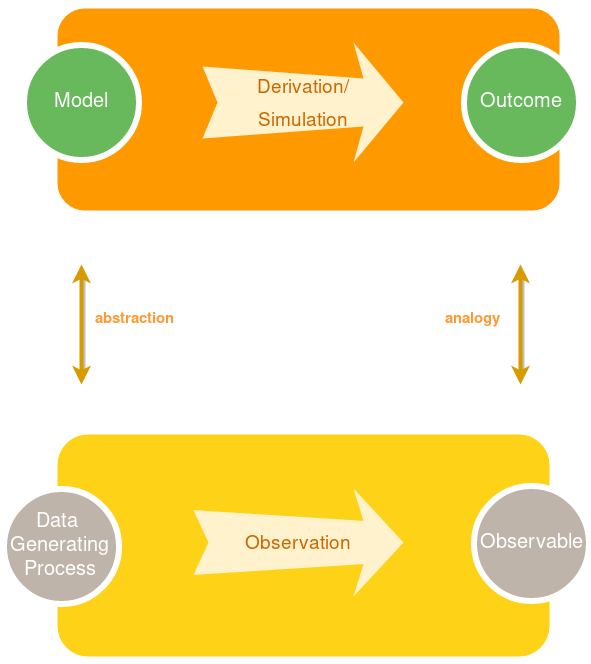
\includegraphics[scale = 0.5]{ims/ms.png}
  \caption{Relação entre Modelos e Sistemas Alvo.}
  Fonte: Adaptado de \citeonline{downey2012think}
\end{figure}

O estudo formal da ação e escolha coletiva teve como período de fundação moderno
o período entre \citeonline{black1948rationale} (marco no estudo da escolha coletiva)
e \citeonline{olson1965logic} (marco para os estudos da ação coletiva), embora
\textit{insights} típicos da literatura, como paradoxos da agregação ou o
problema do caroneiro, tenham sido discutidos anteriormente por pensadores como
Plínio, o Jovem (64-114 d.C.); Ramon Lull (1232-1315); David Hume; e John Stuart
Mill \cite{mclean2015strange, sep-free-rider, ordeshook1990emerging}. 


Embora não seja a única forma de se modelar formalmente fenômenos políticos,
modelos de escolha racional são em larga medida os mais comuns
\cite{austen1998social}. De uma forma geral, os modelos da Teoria da Escolha
Racional, em política, buscam representar fenômenos segundo alguma variante da
seguinte equação, a Equação de Plott \cite{munger2015choosing,
  ostrom1986agenda}\footnote{Essa ``equação'' é conceitual. \(\oplus\) é usado como
  um operador abstrato não especificado \cite{ostrom1986agenda}. }:
\begin{figure}[H]
\begin{align*}
  \text{Preferences} \oplus \text{Beliefs}  \oplus  \text{Physical Possibilities} \oplus \text{Institutions} = \text{Outcomes}
\end{align*}
\end{figure}
O conjunto de modelos conhecidos como ``Teoria da Escolha Racional'' podem ser
dividido em duas variantes: \textit{thin} ou \textit{thick}
\cite{hechter1997sociological, green1996pathologies}. Ambos os tipos de modelos
são construídos com base nos pressupostos mínimos de um modelo de ator racional:
preferências racionais e racionalidade bayesiana \cite{gintis2016individuality}.
A diferença entre eles é que os modelos \textit{thin} não fazem pressupostos
substantivos sobre os valores e objetivos dos agentes. Neles os teóricos buscam
modelar a combinação entre agentes e instituições da maneira mais geral
possível. Já modelos \textit{thick} adicionam um conjunto de pressupostos extras
sobre objetivos, valores, incerteza, com o objetivo de representar fenômenos
particulares como o comparecimento às urnas, a competição partidária, a escolha
de candidatos pelo eleitorado, independência burocrática, o efeito fiscal de
constituições, dentre outros \cite{bendor2011behavioral}.

Todo modelo formal da escolha racional em política envolve os seguintes
elementos primitivos: o conjunto $N$ de agentes, o conjunto \(X\) de
alternativas possíveis, e para cada agente em \(N\) uma descrição de suas
preferências em relação às alternativas em \(X\) \cite[p.
263]{austen1998social}.

A preferência é uma relação de comparação de valor, onde dois conceitos são
fundamentais: o de melhor (preferência estrita), denotado por \(\succ\) e o de igual
em valor (indiferença), denotado por \(\sim\). As seguintes propriedades definem a
noção lógica de relação de preferência \cite{sep-preferences}:

\begin{enumerate}
\item \textit{Assimetria da preferência}: \( x \succ y \to \neg (y \succ x )\); 
\item \textit{Simetria de indiferença}: \(x \sim y \to  y \sim x\); 
\item \textit{Reflexividade da indiferença }: \(x \sim x\); 
\item \textit{Incompatibilidade entre preferência e indiferença}: \(x \succ y \to \neg ( x
  \sim y)\).
\end{enumerate}

A relação de preferência fraca \( \succeq \)pode ser definida da seguinte forma:

\begin{align*}
  \text{x} \succeq y \leftrightarrow x \succ y \lor x \sim y
\end{align*}

A aplicação dessa definição de preferência no modelo do ator racional pressupõe
que ela seja uma relação binária no conjunto de alternativas \(X\), com as
seguintes propriedades, para todo \(x,y,z\) $\in$ \(X\), e para todo conjunto
\(Z\) $\subset$ \(X\) \cite{gintis2016individuality,
  binmore2008rational}:



\begin{enumerate}
\item \textit{Completude}: \(\{ x \succeq y | \vspace{0.4cm} X \}\) ou \(\{ y \succeq x |
  \vspace{0.4cm} X \}\);
\item \textit{Transitividade}: \( \{x \succeq y | \vspace{0.4cm} X\} \) e \(\{y \succeq z |
  \vspace{0.4cm} X \}\) tem por implicação \(\{x \succeq z | \vspace{0.4cm} X\}\);
\item \textit{Independência das alternativas irrelevantes}: para \(x,z \in Z\),
  \(\{x \succeq y | \vspace{0.4cm} Z \}\) se e somente se \(\{x \succeq y | \vspace{0.4cm}
  X\}\).
\end{enumerate}

Um pressuposto adicional é que existe um \(x \in X\) tal que para todo \(y \in X\),
\(x \succeq y\), e que num ambiente sem restrição os atores escolhem essa alternativa
\cite{gintis2009bounds}. Esses pressupostos constituem o primeiro princípio do
modelo do ator racional: os agentes possuem \textit{preferências consistentes ou
racionais}, o que significa que são completas, transitivas e independentes de
alternativas irrelevantes.

Uma conveniência analítica é representar relações de preferência por meio de
funções de utilidade, que são funções que atribuem um número real para cada
elemento do conjunto de alternativas \cite{sep-preferences}. A relação \( \succeq\) é
representada pela função \(u\): \(X \longrightarrow \mathbb{R}\) se e somente se:

\begin{align*}
  u(x) \geq u(y)
  \text{ se e somente se }
  x \succeq y
\end{align*}

Por meio dessa representação, a alternativa preferida, ou ótima, para um ator $i
\in N$ é dada por \cite{binmore2008rational}:
\[\max_{\substack{x \in  X}}
  u_i(x)
\]

Importante notar que funções de utilidade são um dispositivo matemático. Modelar
agentes por meio de funções de utilidade 
não implica que eles sejam  egoístas, instrumentais, utilitários,
hedonistas, ou que estejam ``tentando maximizar sua utilidade''
\cite{gaus2007philosophy}.

O segundo princípio dos modelos de ator racional é a \textit{racionalidade
  bayesiana} \cite{gintis2016individuality}. Quando as alternativas são
probabilísticas primeiro pressupomos que os agentes tem um \textit{modelo do
  mundo}\cite{acemoglu2011opinion}: os agentes vão ter uma crença, representada
por meio de uma função de distribuição de probabilidade\footnote{O modelo da
  escolha racional então pressupõe que as crenças dos agentes são coerentes ou
  consistentes, o que equivale a dizer que estão em conformidade com os axiomas
  da probabilidade \cite{jackman2009bayesian}.}, a qual vai atribuir uma
probabilidade \(p\) para cada evento em \(X\). A partir disso pressupõe-se que
agentes vão ter uma relação de preferência sobre
\textit{apostas}\cite{jehle2001advanced}, onde o conjunto de apostas
\(\mathcal{G}\) em \(X = \{ x_1, \ldots, x_n \}\) é dado por:

\begin{align*}
  \mathcal{G} \equiv \big{\{}  (p_1 \circ x_1, \ldots, p_n \circ x_n  ) | p_i \geq 0, \sum_{i = 1 }^n p_i = 1  \big{\}}  
\end{align*}

Sendo assim, quando as alternativas são probabilísticas o modelo do agente
racional pressupõe que os agentes vão ter uma função de utilidade esperada \(u:
\mathcal{G} \to \mathbb{R} \):

\begin{align*}
  u(\mathcal{G}) = \sum_{i =1}^n p_i u(x_i)
\end{align*}

O último elemento do princípio da \textit{racionalidade bayesiana} é a
\textit{atualização bayesiana}\cite[p.104]{gintis2016individuality}: os agentes
atualizam suas crenças segundo a Regra de Bayes.

Sendo assim, os modelos de escolha racional na sua versão mais básica pressupõem
agentes com preferências consistentes, o que implica que sejam transitivas,
completas e independente de alternativas irrelevantes. Caso o contexto de
decisão seja incerto também pressupõem que os agentes tem uma crença em
conformidade com os axiomas da probabilidade, agem de acordo com princípio da
utilidade esperada e atualizam suas crenças de acordo com o Teorema de Bayes.



\section{Teoria Política Espacial}
 











